\chapter{OpenDQ introduction}
\label{sec:01-introduction}
OpenDQ is an open source project started in 2014 by OpenMote Technologies that implements a MAC (Medium Access Control) protocol targeted at data collection scenarios using low-power wireless technologies, i.e., active RFID (RadioFrequency IDentification) or WSN (Wireless Sensor Networks).

In a data collection scenario, as depicted in Figure~\ref{fig:01-architecture}, there are three types of devices; a computer, a gateway and the nodes. The nodes are computing devices equipped with a low-power wireless radio transceiver to communicate, various analog or digital sensors to acquire data from the environment and, finally, batteries that provide energy to the whole system. In a given scenario, i.e., a warehouse, the combination of the sensing, computing and communication capabilities of such devices allows to collect measurements of physical parameters, i.e., temperature or relative humidity, in a distributed manner. The acquisition of data by nodes can be performed periodically, i.e., every minute, or on demand, but the collection of data is always performed on demand. Thus, the role of the gateway is to trigger the collection process to obtain the information of all nodes that are within its communication range and to provide such information to the computer. Since the coverage may be limited due to wireless propagation or interference conditions, one or more gateways are typically deployed in a given scenario to ensure that all nodes can be collected appropriately. Finally, the computer is responsible trigger the data collection process and to collect and store the data provided by the gateway(s), as well as to provide it to third parties.

% A data collection scenario
\begin{figure}[!t]
    \centering
	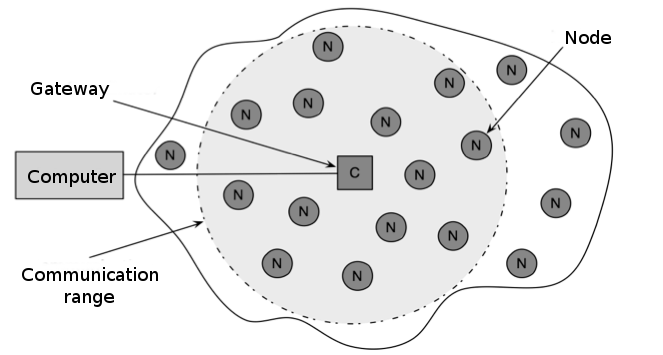
\includegraphics[width=0.75\linewidth]{01-architecture}
    \caption{A data collection scenario}
    \label{fig:01-architecture}
\end{figure}

Since nodes are battery-powered computing devices that communicate using low-power wireless technologies, the data collection scenarios described above presents three main challenges:
\begin{itemize}
\item First, the number of nodes that may be present within the gateway communication range may be large, i.e., hundreds to thousands.
\item Second, the number of nodes that may be present within the gateway communication range is unknown a priori, i.e., because nodes are mobile.
\item Third, the traffic patterns generated by the nodes in the data collection phase is bursty, i.e., all nodes transmit their data simultaneously.
\end{itemize}

Given the above scale, mobility and traffic pattern constraints, existing MAC protocols targeted at data collection scenarios are not suitable. On the one hand, TSCH (Time Synchronized Channel Hopping), as defined in IEEE~802.15.4e \cite{ieee802.15.4e}, is not suitable because it assumes that nodes are statically deployed in a given location and cannot cope with bursty traffic patterns. On the other hand, FSA (Frame Slotted ALOHA), as defined in ISO~18000-7:2009 \cite{iso18000-7:2009}, is not suitable because it is not able to cope with a large number of devices and the bursty traffic patterns.

Considering the limitations of existing MAC protocols for data collection scenarios, OpenMote Technologies has developed the OpenDQ project. OpenDQ implements a MAC protocol that combines a packet-based PS (Preamble Sampling) mechanism with a DQ (Distributed Queuing) channel access mechanism. On one hand, the packet-based PS mechanism provides the means for the gateway to synchronize an indeterminately large number of nodes that are within its communication range to trigger the data collection process. On the other hand, DQ is responsible to manage access to the wireless channel to ensure that data from all the nodes present within the gateway communication range can be collected efficiently in terms of time and energy regardless of the number of nodes present in the gateway communication range\footnote{For comparison purposes, the OpenDQ project also implements FSA (Frame Slotted ALOHA).}.

Currently, the OpenDQ project is implemented using OpenMote hardware platform, which is based on a ARM Cortex-M3 micro-controller and a 2.4~GHz radio transceiver compatible the IEEE~802.15.4 standard \cite{ieee802.15.4-2006}. However, the OpenDQ project can be easily ported to other computer architectures, i.e., MSP430, and low-power wireless communication technologies, i.e., Sub-GHz. The only constraint is that the implementation needs to be compliant with existing regulation for unlicensed bands, i.e., FCC in the US \cite{fcc} or ETSI in Europe \cite{etsi}.

The remainders of this document assumes a certain knowledge of MAC protocols for WSN and RFID, as well as PS protocols, FSA and DQ. Thus, for readers not familiar with the related topics it is advised to have a look at the following references.

For an introduction to MAC protocols for WSN and RFID have a look at the following references:
\begin{itemize}
\item "Dheeraj K Klair, Kwan-Wu Chin, and Raad Raad. A survey and tutorial of RFID anti-collision protocols. Communications Surveys \& Tutorials, IEEE, 12(3):400–421, 2010. \cite{Klair2010}
\item A Bachir, M. Dohler, T. Watteyne, and K K Leung. MAC essentials for wireless sensor networks. Communications Surveys \& Tutorials, IEEE, 12(2):222–248, 2010. \cite{Bachir2010}.
\item P Huang, L. Xiao, S Soltani, M Mutka, and N Xi. The Evolution of MAC Protocols in Wireless Sensor Networks: A Survey. Communications Surveys \& Tutorials, IEEE, (99):1–20, 2012. \cite{Huang12}.
\end{itemize}

For a survey on PS protocols have a look at the following reference:
\begin{itemize}
\item Cristina Cano, Boris Bellalta, Anna Sfairopoulou, and Miquel Oliver. Low energy operation in WSNs: A survey of preamble sampling MAC protocols. Computer Networks, 55(15):3351–3363, 2011. \cite{Cano2011}.
\end{itemize}

Finally, for references related to the DQ channel access mechanism have a look at:
\begin{itemize}
\item W. Xu and G. Campbell. A near perfect stable random access protocol for a broadcast channel. In Communications (ICC), 1992 IEEE International Conference on, pages 370–374, 1992. \cite{Xu1992}.
\item W. Xu and G. Campbell. A distributed queueing random access protocol for a broadcast channel. SIGCOMM Comput. Commun. Rev., 23(4):270–278, 1993. \cite{Xu1993}.
\item L. Alonso, R. Agusti, and O. Sallent. A near-optimum MAC protocol based on the distributed queueing random access protocol (DQRAP) for a CDMA mobile communication system. Selected Areas in Communications, IEEE Journal on, 18(9):1701–1718, 2000. \cite{Alonso2000}.
\item J. Alonso-Zarate, C. Verikoukis, E. Kartsakli, A. Cateura, and L. Alonso. A near-optimum cross-layered distributed queuing protocol for wireless LAN. Wireless Communications, IEEE, 15(1):48–55, 2008. \cite{Alonso2008}.
\item Pere Tuset, Francisco Vazquez, Jesus Alonso, Luis Alonso, and Xavier Vilajosana. LPDQ: a self-scheduled TDMA MAC protocol for one-hop dynamic low-power wireless networks. Elsevier Pervasive and Mobile Computing, Special Issue on “Internet of Things”, 2014. \cite{Tuset2014a}.
\item Pere Tuset, Francisco Vazquez, Jesus Alonso, Luis Alonso, and Xavier Vilajosana. Experimental energy consumption of FSA and DQ for data collection scenarios. MDPI Sensors, Special Issue on “Wireless Sensor Networks and the Internet of Things”, (14):13416–13436, 2014. \cite{Tuset2014b}.
\end{itemize}